\section{Designing a Classifier}
To understand the processes involve in user engegement with a micro video, we designed an experinmen where in we use machine learning methods,  to understand influence of the features used for training, on the engagement classification process. By doing so we would be able to understand the relevance of different kinds of features on the overall engagement potential of a micro video and gain some empirical evidence about the impact contribution by each Aesthetic, Audio, contextual and social features. Further to validate our hypothesis about differential impact of the initial seconds on the engagement against the rest of the video, we train two classifiers where one uses the features across the complete video, and other only the first 2 seconds. Comparing the performances of both, we were able to conclusively propose the validity of our hypothesis.  
\par
Due to the exhastive nature of our data, the computational resources in terms of CPU usage and time would be unmanagable, so we sampled 18,000 videos from our datasets to work with. Out of thes 18,000  6,000 videos were sampled from the POP12K gold standard dataset which contain all high engagement videos. Addional 12,00 videos were sampled from the broadly sampled UNPOP120K dataset. These videos mostly fall towards the lower end of engagement. These videos were then sampled for individual frames every second and processed to extract the 28 dimentional vector of all the contextual, perceptual , aesthetic features.  Audio features were seperately extracted from the audio track and social fearures from the post metadata. To get a better understanding of the dimensionality and ordering of the features refer to Table \ref{tab:Features_table}. The classifier is binary, so it only tells us if a video is engaging or not for a given definition of "Engaging". Using this as a criteria, we vary our definition of "Engaging" by changing the threshold of Loop count, at which a video is labelled as engaging. This threshold is varied from median loop count of ALL120K dataset all the way till 1.5 times Median of POP12K dataset. So in a nutshell, we make our definition of what classifies as engaging, more and more selective. The classifier is trained using cross validated dataset, which is devided in 80\% for training and 20\% for testing. The training process is interated across the range of engagement threshold criteria , 30 times, and in each iteration the performance and the impact of individual features is noted. The Fig \ref{fig:Feature_importance} shows the variation of the impact of social features, compared with all the other content related features across all the iterations. It is important to note, that the impact of content related features, become more decisive as we make our engagement criteria more selective. 


\begin{figure}[!htb]
\centering
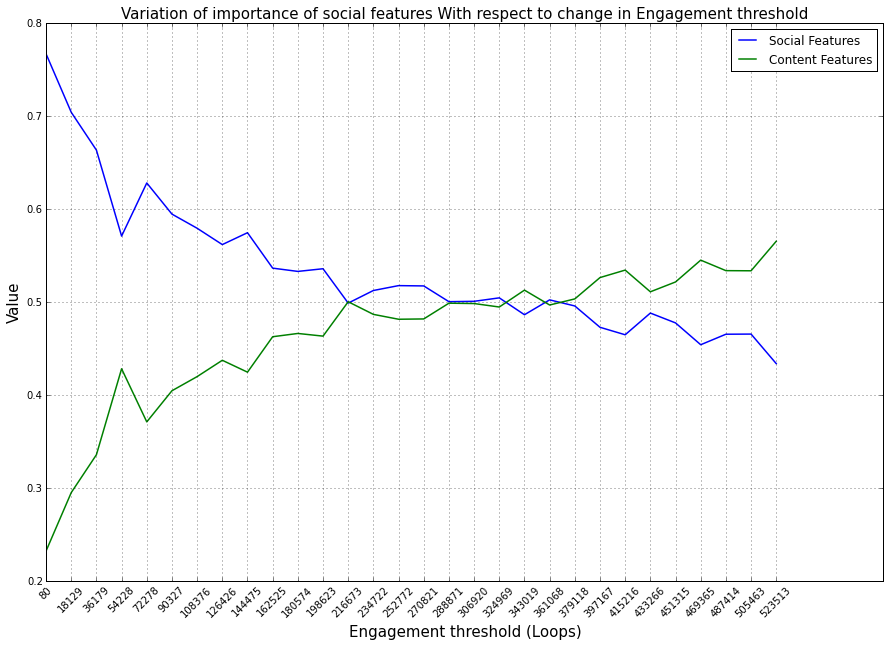
\includegraphics[width=\columnwidth]{plots/EngagementFeatureImpact}
\caption{\textsl{ A plot of contribution of social features against all the perceptual features combined. The influence is calculated by training the classifier and looking at the coeeficients of the final function. The values are generated by interating the training and testing process for different thresholds for the definition of a popular post. The x axis signifies the threshold value of Likes at which a video is labelled to be popular. It starts from the median of the UNPOP120K and ends at 1.5 times the median of POP12K. }}
\label{fig:Feature_importance}
\end{figure}



\begin{figure}[!htb]
\centering
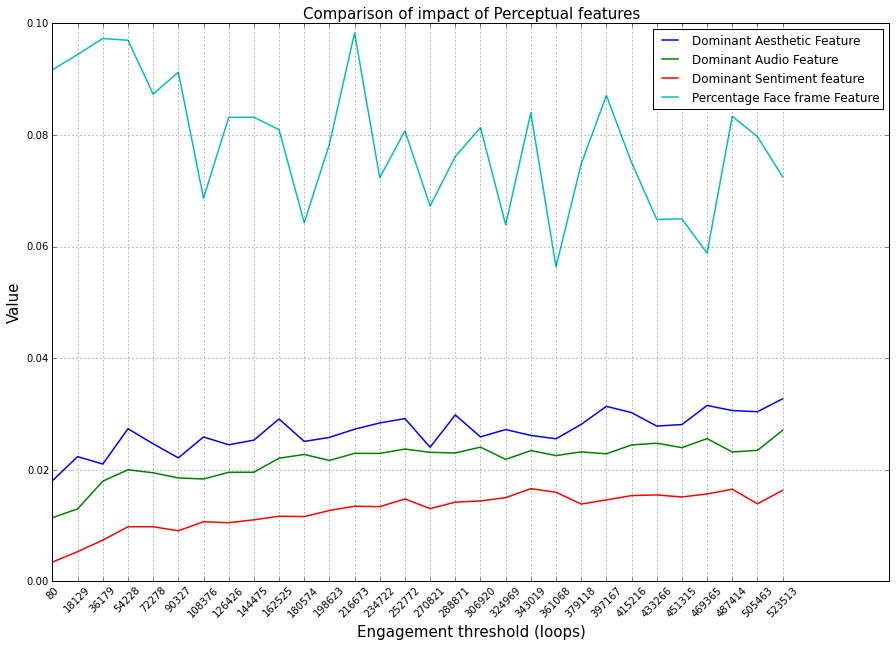
\includegraphics[width=\columnwidth]{plots/EngagementContentFeatureImpact}
\caption{\textsl{ The plot shows change in impact of individual track features as we become more selective. The most prominent features among the content features is the presence of face. }}
\label{fig:Feature_importance_content}
\end{figure}


\begin{figure}[!htb]
\centering
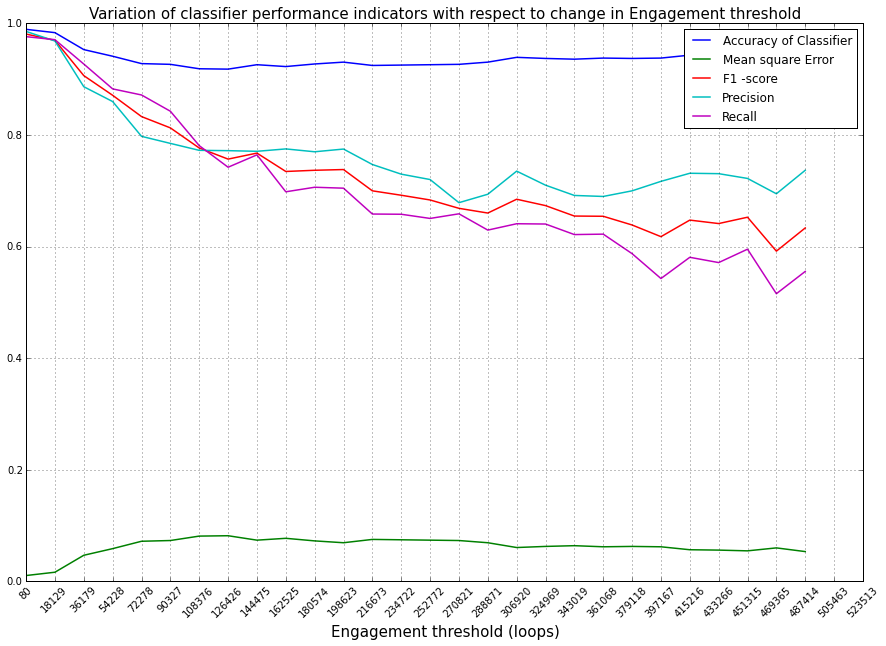
\includegraphics[width=\columnwidth]{plots/EngagementClassifierPerf}
\caption{\textsl{ The plot shows varying values of Precision, Recall, Accuracy and F1-score across the classifier traning iterations}}
\label{fig:Classifier_performance}
\end{figure}
 
Now to further verify the theory about the importance of first seconds in vine, we trained the whole classifier setup over the same dataset. The major difference this time was that the features were now extracted from the frames sampled from the first two seconds of the vine. \sj{HERE AFTER WE SHOW THAT THE PERFORMACE IS THE SAME OR DEGRADED MARGINALLY}